\documentclass{article}
\usepackage{amsmath, amssymb}
\usepackage{tikz}
\usetikzlibrary{arrows.meta, positioning, shapes}

\begin{document}

\title{Proof: \( 8 \) Divides the Difference of Squares of Two Odd Numbers}
\maketitle

\section{Theorem}
Let \( a \) and \( b \) be odd integers. Then:
\[
    8 \mid (a^2 - b^2)
\]

\section{Proof}
We prove this by expressing odd numbers in their general form and simplifying.

\subsection{Step 1: Representation of Odd Numbers}
Any odd integer can be written as:
\[
    a = 2k + 1, \quad b = 2m + 1 \quad \text{where } k, m \in \mathbb{Z}.
\]

\subsection{Step 2: Compute \( a^2 - b^2 \)}
Using the difference of squares:
\[
    a^2 - b^2 = (a - b)(a + b).
\]
Substitute \( a \) and \( b \):
\[
    a^2 - b^2 = (2k + 1 - 2m - 1)(2k + 1 + 2m + 1) = 2(k - m) \cdot 2(k + m + 1).
\]
Simplify:
\[
    a^2 - b^2 = 4(k - m)(k + m + 1).
\]

\subsection{Step 3: Divisibility by 8}
We show that \( 4(k - m)(k + m + 1) \) is divisible by 8:
\begin{itemize}
    \item **Case 1**: If \( k - m \) is even, then \( (k - m) = 2n \) for some \( n \in \mathbb{Z} \). Thus:
          \[
              a^2 - b^2 = 4(2n)(k + m + 1) = 8n(k + m + 1).
          \]
    \item **Case 2**: If \( k - m \) is odd, then \( k + m + 1 \) must be even (since the sum of an odd and even term is even). Let \( k + m + 1 = 2n \). Thus:
          \[
              a^2 - b^2 = 4(k - m)(2n) = 8n(k - m).
          \]
\end{itemize}
In both cases, \( a^2 - b^2 \) is divisible by 8.

\subsection{Conclusion}
For any two odd integers \( a \) and \( b \), \( 8 \) divides \( a^2 - b^2 \).


\section{DAG Diagram of the Proof}
\begin{center}
    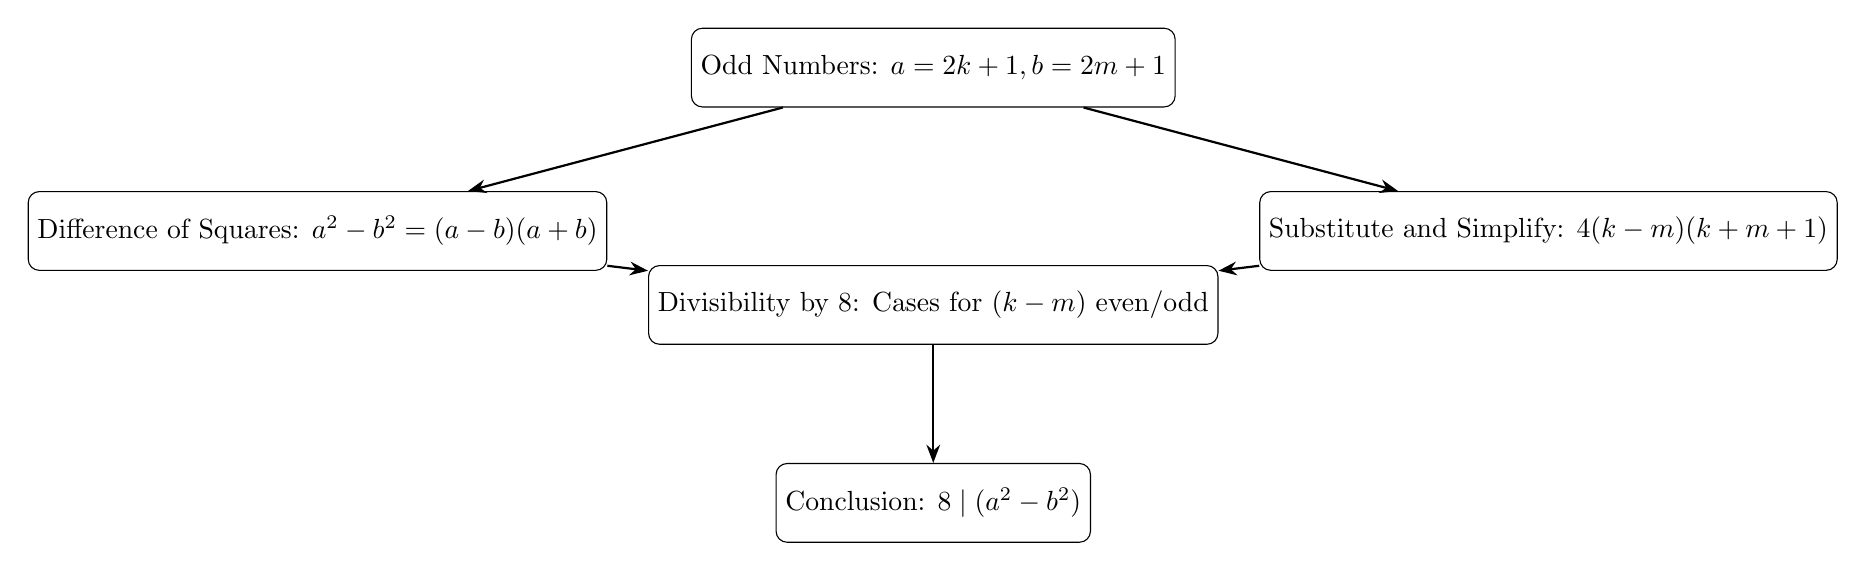
\begin{tikzpicture}[
            node distance=1.5cm,
            box/.style={draw, rectangle, rounded corners, minimum width=2.8cm, minimum height=1cm, text centered},
            arrow/.style={-Stealth, thick},
            scale=0.2 % Scale the entire diagram to 80% of its original size
        ]

        % Nodes
        \node[box] (odd-def) {Odd Numbers: \par \( a = 2k+1, b = 2m+1 \)};
        \node[box, below left=of odd-def] (diff-sq) {Difference of Squares: \par \( a^2 - b^2 = (a-b)(a+b) \)};
        \node[box, below right=of odd-def] (substitute) {Substitute and Simplify: \par \( 4(k-m)(k+m+1) \)};
        \node[box, below=2cm of odd-def] (divisibility) {Divisibility by 8: \par Cases for \( (k-m) \) even/odd};
        \node[box, below=of divisibility] (conclusion) {Conclusion: \par \( 8 \mid (a^2 - b^2) \)};

        % Arrows
        \draw[arrow] (odd-def) -- (diff-sq);
        \draw[arrow] (odd-def) -- (substitute);
        \draw[arrow] (diff-sq) -- (divisibility);
        \draw[arrow] (substitute) -- (divisibility);
        \draw[arrow] (divisibility) -- (conclusion);

    \end{tikzpicture}
\end{center}

The DAG illustrates:
\begin{itemize}
    \item The **definition of odd numbers** leads to algebraic manipulation.
    \item The **difference of squares** and **substitution** steps converge.
    \item **Divisibility by 8** is shown by case analysis.
    \item The **conclusion** follows from the cases.
\end{itemize}

\end{document}